\documentclass[letterpaper, 12 pt]{article} %Modifica el tipo de documento y el tamaño de la letra.
\usepackage[utf8]{inputenc} %Formato UTF-8 para caracteres especiales.
\usepackage[shortlabels]{enumitem}
\usepackage[spanish,mexico]{babel} 
\usepackage{amsmath,amssymb,amsfonts,latexsym,cancel}
\usepackage{hyperref}
\usepackage{wrapfig}
\usepackage[rflt]{floatflt}
\usepackage[pdftex]{graphicx}
\usepackage{fancyhdr} %Paquete para el header y el formato de la portada. No sugiero borrarlo!
\usepackage{float}
\usepackage{longtable,multirow,booktabs}
\usepackage{cite}
\usepackage{wrapfig}
%\usepackage[square,numbers]{natbib}
\usepackage{multicol}
\usepackage{caption}
\usepackage[]{sidecap}
\usepackage{adjustbox}
\usepackage{parskip}
\usepackage{enumitem}
\usepackage{tikz}
\usepackage{lipsum}
\usepackage[]{xcolor}
\usepackage[style=ieee]{biblatex}
\addbibresource{Libros.bib}

%\usepackage[showframe]{geometry}
%\geometry{margin=1cm, top=1cm, headsep=1cm, footskip=1cm}

%Inicio formato de Página. Puedes establecer medidas de la página y modificar el header.

\textheight = 21cm %Medidas de la  página
\textwidth = 18cm  %Medidas de la página
\topmargin = -2cm  %Medidas de la página    
\oddsidemargin = -0.8cm %Medidas de la página
%\pagestyle{fancy} %Diseño de la página

%\fancyhf{}
\lhead{Facultad de Ingeniería}%%LeftHead
\chead{
\includegraphics[width=1cm, height=1cm]{Imágenes/UNAM.png}}%%CenterHead
%\lfoot{USM}
\rhead{Sistemas Operativos Grupo: 06}%%RightHead

\setlength{\columnsep}{4mm}%Comandos para el formato de la página.
%\setlength{\parindent}{4em}%Sangría al comenzar un nuevo párrafo.
\setlength{\parindent}{0.5in}
%\setlength{\parindent}{4em}%Sangría al comenzar un nuevo párrafo.
\setlength{\parskip}{1em}%Distancia entre párrafos.
\renewcommand{\baselinestretch}{1.5}% Espacio entre línea y línea o interlineado.
\setlength{\headheight}{33pt}
\fancyfoot[CE,CO]{\\\thepage} %Logo de LaTeX y pie de página. \LaTeX{}

%\documentclass{report}
\usepackage{tabularx}
\usepackage{pgf}
\usepackage{pgfpages}
%\usepackage{bold-extra}
%\usepackage{charter}
\usepackage{xcolor}


\definecolor{my_chosen_color}{RGB}{0,0,0} %\definecolor{my_chosen_blue}{RGB}{54,131,179}

% Set margin borders

\pgfpagesdeclarelayout{boxed}
{
  \edef\pgfpageoptionborder{0.45cm}
}
{
  \pgfpagesphysicalpageoptions
  {%
    logical pages=1,%
  }
  \pgfpageslogicalpageoptions{1}
  {
    border code=\pgfsetlinewidth{3 pt}\pgfsetstrokecolor{my_chosen_color}\pgfstroke,%
    border shrink=\pgfpageoptionborder,%
    resized width=.95\pgfphysicalwidth,%
    resized height=.95\pgfphysicalheight,%
    center=\pgfpoint{.5\pgfphysicalwidth}{.5\pgfphysicalheight}%
  }%

}

\pgfpagesuselayout{boxed}

%Fin formato de Página

%Aquí inicia el documento. Date como magnate
\begin{document}

    %LaTeX te hace el índice automáticamente conforme añades secciones en tu documento.
    %\thispagestyle{empty}
			\begin{figure}[ht]
		   \minipage{0.87\textwidth}
				
\includegraphics[width=2cm]{Imágenes/inge.eps}
				\label{escudoFI}
		   \endminipage
		   \minipage{0.32\textwidth}
				
\includegraphics[height = 2.25cm ,width=2cm]{Imágenes/UNAM.png}
				\label{EscuoUNAM}
			\endminipage
				%%\vspace{-1cm}
		\end{figure}
		
		\vspace{0.1cm}
		
		\begin{center}
		    {\scshape\LARGE \textbf{Universidad Nacional Autónoma de México} \par}
			{\scshape\Large Facultad de Ingeniería\par}
            
             {\LARGE Electricidad y Magnetismo (L+) (Cve: 6414)}

			% Restauramos el interlineado:
			\begin{center}
			
			{\LARGE Grupo: 20 - Semestre: 2023-2}

            
                %{\LARGE  \bfseries{Cuestionario Previo: xX} \\}
			{\LARGE\bfseries Práctica de laboratorio: 10 \\ Fuerza de origen magnético \\ sobre conductores \par}

		{\scshape\Large Fecha de entrega: 17/05/2023 17:15 hrs \par}	
		% {\scshape\Large Fecha de elaboración: 09/05/2023 09:00 hrs \par}	

			        \LARGE	{ \textbf{Profesor:}}\\%% \textbf son negritas
        \large		{ Dr. Germán Ramón Arconada Rey }
        %\large		{ Reposición de práctica:  }
        % \large		{ Juárez de la mora Lucía Yazmín }
        
		\vspace{-0.5cm}	
		
		\LARGE	{ \textbf{Brigada 05:}}\\%% \textbf son negritas

        \normalsize	 {Arellanes Conde Esteban: 31932274-3}
        
        % \vspace{-0.5cm}
        
        % \normalsize		{Belmont Muñoz Samuel: 31731828-9}
        
        % \vspace{-0.5cm}
        
        % \normalsize		{Carbajal Pacheco Josué: 31931513-6}

        % \vspace{-0.5cm}
        
        % \normalsize		{Esquivel Santana Christian: 31929014-5}

        
        
%% \it es letra itálica
				\vspace{1.25cm}
				\vspace{0.9cm}
				
			\end{center}
	
		\end{center}

  
    %\tableofcontents
    %\newpage
%Inicio parte opcional. Esta parte la puedes quitar si deseas, es por si te piden formatos para
%evidencias de certificación de los laboratorios con números de cuenta o te piden abstracts en tus %trabajos.

\title{\textbf{Sistemas Operativos} \\ Proyecto 01: Revisión de Fascículo 22 \\ MiComputer\\ } 

\author{
  %\normalsize{\texttt{---------}} \and
  \normalsize{\texttt{Arellanes Conde Esteban: 319322743}} \\
  \normalsize{\texttt{Esquivel Santana Christian: 319290145}} \\
  %\normalsize{\texttt{/////////}} \and
  %\normalsize{\texttt{ }} \and
}
\date{\normalsize{\textbf{Fecha límite de entrega:} 05/09/2024 23:59:59 hrs \\ (5 de Septiembre de 2024 a las 23:59)}}
\maketitle
\thispagestyle{fancy}

\begin{center}
\section*{Reseña y Resumen sobre la máquina de Turing, Commodore PET 4032, Color, Sonido, Luz y Jerga Geek:}
\end{center}

\section*{Reseña y Resumen sobre La Máquina de Turing}
El tema de la máquina de Turing me ha llamado siempre la atención desde el momento en el que lo vimos en materias anteriores como lo fue \textit{“lenguajes formales y autómatas”} y bueno, desde el gran centro de atención que ha sido la inteligencia artificial es normal el ver porque empezó a tener todavía mas relevancia en nuestro sector y en nuestros tiempos. 

Es claro que el tema de la máquina de Turing es un tanto abstracto y hasta cierto punto muy difícil de entender pues después de varias materias en donde se hace mención aun no logro entenderla en su totalidad y dudo mucho que esto suceda en un futuro próximo.

Entrando al tema presentado por la revista aquí se nos presenta como el \textit{“mínimo ordenado posible”}, es utilizado para ilustrarnos como los limites teóricos de la computación afectan la informática práctica, permitiéndonos comprender mejor los algoritmos y determinar que problemas pueden ser informatizado. En cuanto a la estructura de la máquina de Turing, la cual contiene una cinta infinita, la cabeza de lectura/escritura y la unidad de control, rápidamente me hizo recordar aquellos videos vistos en los temas introductorios a la materia, así como también estos reflejan la manera en que los sistemas operativos gestionan los procesos y la memoria.

De igual forma, así como la máquina de Turing sigue una serie de instrucciones o \textit{“quíntuplos”} para resolver un problema podemos llevarlo a un paralelismo con los sistemas operativos en donde estos manejan los estados y transiciones de múltiples procesos, asegurándose de que cada uno siga la secuencia de instrucciones de manera correcta.

\section*{Reseña y Resumen sobre la Commodore PET 4032:}
Nos parece fascinante el leer este tipo de revistas que ya tienen un cierto tiempo en donde hablan sobre cosas de esa época o que no eran tan \textit{“viejas”} en ese entonces, es como si fuese una máquina del tiempo. En este caso el tomo 22 habla sobre la Commodore Pet 4032, esta fue una computadora que marca un antes y después ya que es la primer computadora de uso personal y por sus materiales (aunque eso ya lo habíamos visto en la introducción de la clase), pero es lo que resalta en su mayoría el articulo y visto en el aspecto de que este computador fuera \textit{“plug and play”} es relevante en cuanto a los sistemas operativos, en donde el BASIC estaba integrado en la ROM, esto significaba que el sistema operativo estaba listo para usarse en el momento en que la maquina se encendiera, este enfoque prefigura la experiencia de usuario que los sistemas operativos de nuestros tiempos buscan ofrecer: una interfaz intuitiva y un entorno preconfigurado que permite al usuario centrarse en sus tareas sin necesidad de preocuparse por otra cosa.

Pero como en la vida misma en todo podemos aprender de lo bueno pero sobre todo de lo malo y es en esta última parte del escrito en donde destaca también esta importancia de ver sistemas operativos y es la \textit{“aislación”} que tuvo el PET debido a las dificultades que se tuvo para convertir programas de y hacia otras plataformas, en donde un sistema operativo moderno no solo basta con ser funcional y eficiente también debe ser flexible y capaz de integrar nuevas tecnologías y de interactuar con otros sistemas de forma fluida. El cual el PET, aunque fue innovador para la época esta limitante hizo que quedará en su propio nicho lo cual afecto en su impacto.

\section*{Reseña y Resumen sobre el Color, Sonido, Luz y Jerga Geek:}
Y por último, aunque no menos importante, el mismo fascículo nos muestra un avance en el tiempo de la evolución de diferentes tecnologías y su impacto en la sociedad, como el uso del término \textit{“Bug"} descubierto por Grace Hopper. Este término, que originalmente se refería a un error físico en los circuitos de las primeras computadoras, ha evolucionado para denotar cualquier tipo de error o defecto en el software. Además, el fascículo explora cómo términos técnicos como \textit{“debugging”} y \textit{“hardware”} han permeado la cultura general, destacando la forma en que el lenguaje técnico se ha integrado en el vocabulario cotidiano y ha influido en la manera en que entendemos y interactuamos con la tecnología moderna.

%\begin{figure}[h!]
%    \centering
%    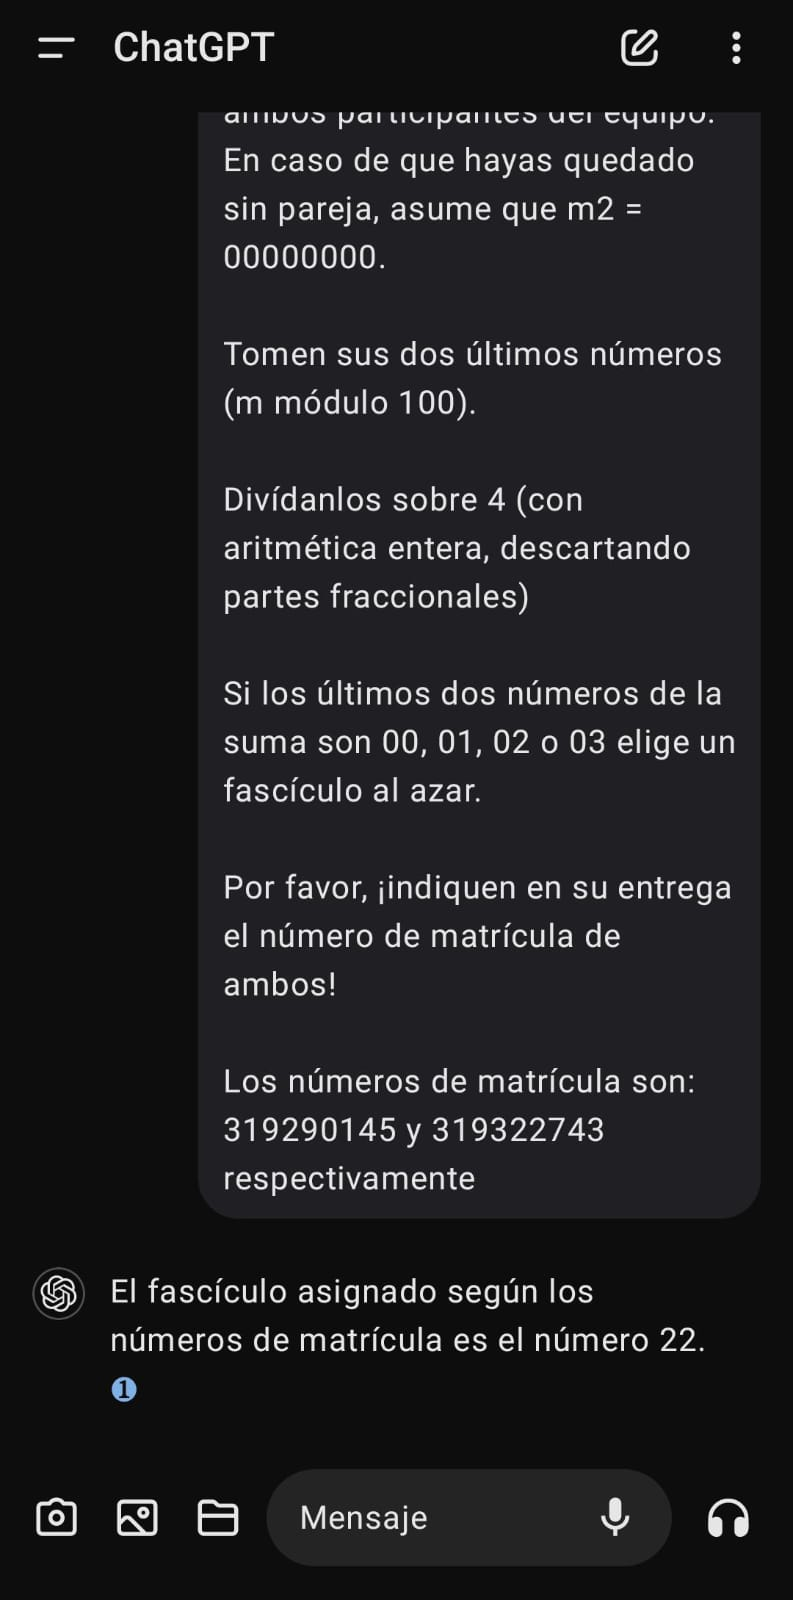
\includegraphics[width=0.5\linewidth]{Imágenes/ScreenShot_Sorteo.jpg}
%    \caption{Sorteo de fascículo}
%    \label{fig:enter-label}
%\end{figure}


\subsection*{Bibliografía}

    %\printbibliography[heading=none]
    \nocite{*}
    \begin{enumerate}[label = \textbf{•}]
        \item Editorial Delta. (1984). MiComputer: Enciclopedia por fascículos semanales (Fascículo 22). Editorial Delta. Consultado de: \url{https://archive.org/details/The_Home_Computer_Course}

        Editorial: Editorial Delta
        Título original: Home Computer Course (publicado por Orbis Publishing)
        Idioma: Español
        Tipo de publicación: Enciclopedia por fascículos semanales
        Número de fascículos: 96 (divididos en 8 tomos)
        Tomos extra: 2 (tomos 9 y 10, traducción de Advanced Home Computer Course)
        Primer número: enero de 1984
    \end{enumerate}
    
\end{document}

 %Fin del documento.